\chapter{Arhitektura i dizajn sustava}

		\section{Arhitektura sustava}
		\begin{figure}[H]
			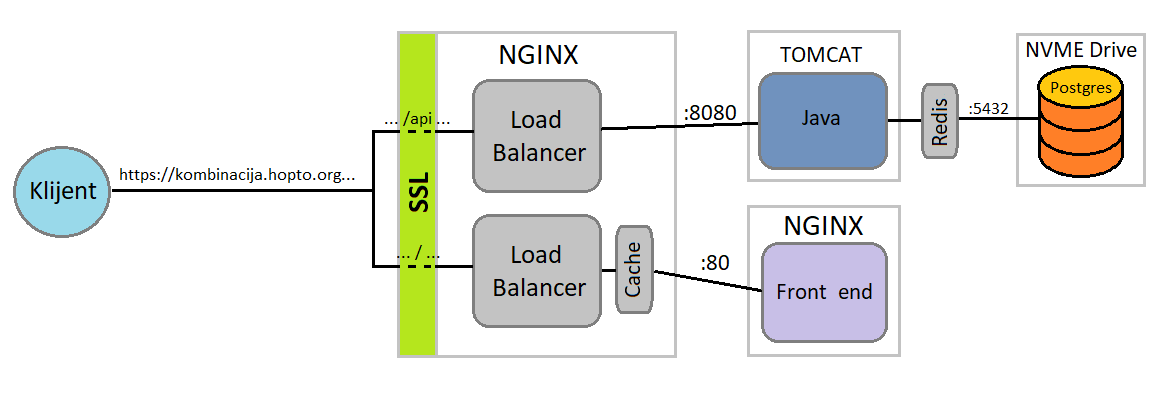
\includegraphics[scale=0.5]{figures/system-architecture.png}
			\centering
			\caption{Arhitektura sustava}
			\label{fig:sys-arch}
		\end{figure}
	
		Slika prikazuje arhitekturu svih sustava, odnosno način na koji su svi dijelovi aplikacije međusobno povezani te način na koji korisnik s njima interagira.
		U cjelokupnom sustavu prepoznaju se sljedeći entiteti i podsustavi:
		\begin{packed_item}
			\item \textbf{Klijent} - putem preglednika šalje HTTPS zahtjeve aplikaciji
			\item \textbf{1. NGINX} - poslužitelj koji šalje i prima HTTPS zahtjeve, a sadrži dva \textit{Load Balancer-a} i \textit{cache} statičkih resursa (\textit{HTML, JavaScript, CSS})
			\item \textbf{2. NGINX} - poslužitelj na kojem se nalazi \textit{front end} aplikacije
			\item \textbf{Tomcat} - poslužitelj na kojem je pokrenuta \textit{Spring} aplikacija
			\item \textbf{Redis} - \textit{cache} između aplikacije i baze podataka
			\item \textbf{NVME Drive} - poslužitelj na kojem je pokrenuta PostgreSQL baza podataka
		\end{packed_item}
	
		Klijent koristeći URL aplikacije - \url{https://kombinacija.hopto.org} - šalje HTTPS zahtjeve aplikaciji koristeći se pritom nekim web preglednikom. Ti upiti pristižu na \textit{reverse proxy} poslužitelj NGINX koji je osiguran SSL-om, a svojim \textit{Load Balancer-ima} upravlja zahtjevima i raspoređuje ih na točne portove. Pri tome se zahtjevi oblika https://kombinacija.hopto.org/api/... prosljeđuju na port :8080 prema \textit{Tomcat} poslužitelju, a zahtjevi oblika https://kombinacija.hopto.org/... na port :80 prema drugom NGINX poslužitelju.
		Java aplikacija pokrenuta na \textit{Tomcat} poslužitelju putem \textit{Redis cache-a} pristupa PostgreSQL bazi podataka na portu 5432.
		
		Poslužitelji \textit{Tomcat} i \textit{2. NGINX} su \textit{instance}, što znači da se u slučaju preintenzivnog korištenja aplikacije može napraviti dodatni poslužitelj sa jednakim sadržajem, a \textit{Load Balancer-i} će osigurati da se svakom daje podjednak udio zahtjeva. Zbog toga je aplikacija lako skalabilna.
		
		\section{Arhitektura aplikacije}
		Za izradu aplikacije na strani \textit{back end-a} odabrali smo programski jezik Java, koristeći se pritom Spring Boot radnim okvirom koji uvelike olakšava razvoj web aplikacija. Radi lakšeg uključivanja vanjskih biblioteka te radi postizanja neovisnosti o razvojnom okruženju koristimo Maven.
		
		Na strani \textit{front end-a} koristimo radni okvir Bootstrap, pomoću kojeg koristimo standardne jezike za dizajniranje i ponašanje web stranica na strani klijenta - HTML, CSS i JavaScript. Radi jednostavnijeg pisanja, uz \textit{vanilla JavaScript} koristimo i \textit{jQuery} biblioteku, kojom je uvelike olakšano slanje asinkronih (\textit{AJAX}) zahtjeva na web poslužitelj.\\
		\\
		Arhitektura sustava se temelji na konceptu MVC (\textit{Model-View-Controller}), kako bi se što jasnije i smislenije razdvojili pojedini dijelovi aplikacije te omogućio njihov istodoban i neovisan razvoj. 
		\begin{figure}[H]
			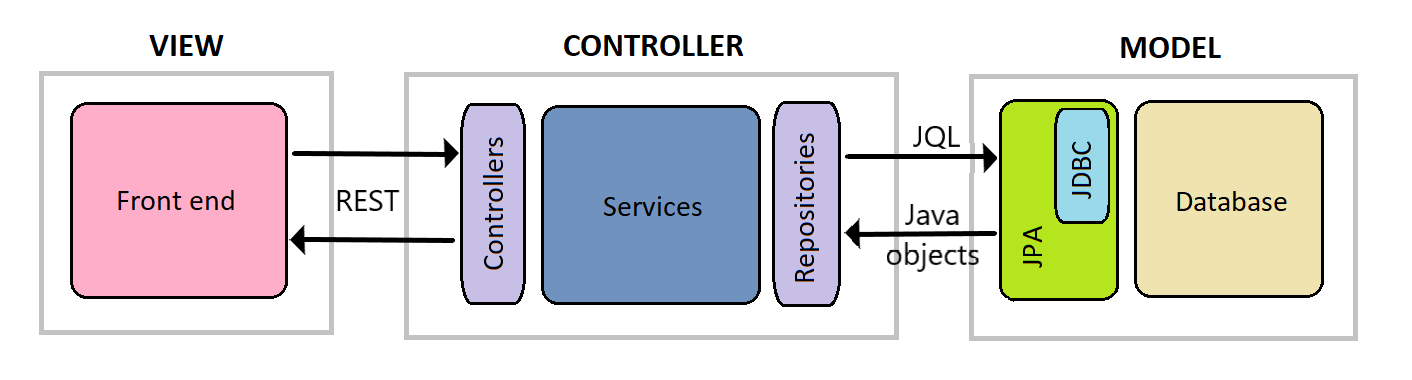
\includegraphics[scale=0.4]{figures/MVC.png}
			\centering
			\caption{MVC prikaz aplikacije}
			\label{fig:mvc}
		\end{figure}
		
		\textbf{View} označava podsustav zadužen za \textit{user-friendly} prikaz podataka korisniku. U slučaju naše aplikacije, razvija se potpuno neovisno od ostalih dijelova, te je pokrenut na zasebnom poslužitelju. Osim što prikazuje \textit{model}, \textit{view} je zadužen i za slanje zahtjeva \textit{controller-u}. 
		
		\textit{View} sa elementom \textit{Front end} se u potpunosti preslikava na prethodnu sliku u poslužitelj \textit{NGINX}, u kojem se također nalazi element \textit{Front end}.\\
		\\
		\textbf{Controller} označava podsustav koji upravlja zahtjevima pristiglim iz \textit{view-a}, dohvaća stvarne podatke iz \textit{model-a} te vrši logiku svih mogućih akcija i događaja. Svi dijelovi \textit{controller-a} se preslikavaju u poslužitelj \textit{Tomcat} sa prethodne slike, a njegov središnji dio predstavljaju servisi, koji se u samoj aplikaciji nalaze u posebnom paketu, a koji obavljaju cjelokupnu poslovnu logiku aplikacije. Kako bi to obavljali uspješno, moraju moći komunicirati sa ostalim podsustavima.
		
		Komunikacija s \textit{view-om} se izvodi putem sučelja \textit{Controllers}, koje na slici predstavlja cijeli paket u kojem je definiran API (\textit{Application Programming Interface}) putem kojeg se aplikaciji šalju zahtjevi ili se dohvaćaju podaci. API koji smo odabrali je REST (\textit{REpresentational State Transfer}) API, kako bi se omogućila lakša komunikacija sa drugim sustavima, te kako bi aplikacija bila lako proširiva (primjerice, na isti API se može spojiti i mobilna aplikacija).
		 
		\textit{Controller} sa modelom komunicira putem sučelja \textit{Repositories} koje također predstavlja cijeli paket kojim se iz baze podataka dohvaćaju konkretne objekte i podatke. Upiti prema bazi se ostvaruju pomoću JQL (\textit{Java Query Language}), oslanjajući se pritom većinom na već implementirane metode uključene u Spring Framework.\\
		\\
		\textbf{Model} predstavlja sve strukture podataka, objekte i zapise vezane uz aplikaciju, koji su spremljeni u bazi podataka. Komunikacija s bazom je ostvarena putem JPA/JDBC specifikacije. Osim JPA, koji se također nalazi na poslužitelju \textit{Tomcat}, \textit{model} se preslikava u disk \textit{NVME Drive} na kojem je pokrenut PostgreSQL server. 

	
		\section{Baza podataka}
			
			Kao sustav upravljanja bazom podataka koristimo PostgreSQL \textit{Sustav za Upravljanje Bazom Podataka} (SUBP). Na bazu se spajamo putem \textit{Java DataBase Connectivity} (JDBC) specifikacije, koja omogućuje Java programima spajanje na SUBP i njegovo korištenje. Na JDBC specifikaciju nadograđuje se \textit{Java Persistence API} (JPA) koji pruža usluge \textit{Object-Relational Mapping} (ORM), čime se odabrani Java objekti automatski spremaju u bazu podataka.
		
			\subsection{Opis tablica}
			
				U bazi podataka nalazi se 9 relacija:
				\begin{packed_item}
					\item \textbf{Persons} - relacija koja opisuje osobu u najširem smislu; osoba može biti korisnik aplikacije, komunalni radnik ili administrator sustava, te se u ovoj relaciji spremaju zajednički atributi tih aktora
					\item \textbf{Admins} - relacija u kojoj se nalaze zapisi svih administratora
					\item \textbf{Employees} - relacija u kojoj se nalaze zapisi svih komunalnih radnika
					\item \textbf{Citizens} - relacija u kojoj se nalaze zapisi svih građana - regularnih korisnika aplikacije
					\item \textbf{Container} - relacija u kojoj su spremljeni zapisi o kontejnerima
					\item \textbf{Neighborhoods} - relacija u kojoj su spremljeni zapisi o susjedstvima
					\item \textbf{Favorites} - relacija u kojoj su spremljeni zapisi o parovima Person-Container, sa značenjem da je osoba Person spremila kontejner Container radi brzog pristupa.
					\item \textbf{Pings} - relacija u kojoj su spremljeni zapisi o parovima Person-Container, sa značenjem da je osoba Person prijavila kontejner Container kao pun, pretrpan ili prazan.
					\item \textbf{Emptyings} - relacija u kojoj su spremljeni zapisi o pražnjenjima kontejnera oblika Employee-Container, sa značenjem da je radnik Employee ispraznio kontejner Container
				\end{packed_item}
			
				Tablica Person je generička tablica za osobu, a nju nasljeđuju tablice Admin, Employee i Citizen, svaki sa svojim dodatnim atributima te stranim ključem koji pokazuje na tablicu Person gdje se nalaze zajednički atributi svojstveni svima trima entitetima.	Tablice Favorites, Pings i Emptyings su tablice koje postoje kako bi se opisala N-N veza između relacija koje povezuju.


			\subsection{Definicije tablica}
			
				U narednim definicijama \textbf{podebljani atributi} označavaju primarne ključeve, a \textit{kurziv} strane ključeve.
				\begin{longtabu} to \textwidth {|X[6, l]|X[6, l]|X[20, l]|}
					
					\hline \multicolumn{3}{|c|}{\textbf{Person}}	 \\[3pt] \hline
					\endfirsthead
					
					\hline \multicolumn{3}{|c|}{\textbf{Person}}	 \\[3pt] \hline
					\endhead
					
					\textit{\textbf{id}} & BIGINT	&   Identifikator osobe; svaka osoba ima svoj jedinstveni ID	\\ \hline
					name	& VARCHAR &   Ime osobe, ne smije biti NULL	\\ \hline 
					last\textunderscore name & VARCHAR & Prezime osobe, ne smije biti NULL \\ \hline
					email & VARCHAR &  E-mail osobe, koristi se pri prijavi korisnika u sustav, ne smije biti NULL i jedinstvena je vrijednost \\ \hline 
					pwd\textunderscore hash & VARCHAR	&  Sažetak lozinke koju je osoba odabrala, ne smije biti NULL \\ 
					\hline
					
					\caption{\label{tab:tbl-person} Tablica \textit{Person}}
					
				\end{longtabu}
			
				\begin{longtabu} to \textwidth {|X[6, l]|X[6, l]|X[20, l]|}
					
					\hline \multicolumn{3}{|c|}{\textbf{Admin}}	 \\[3pt] \hline
					\endfirsthead
					
					\hline \multicolumn{3}{|c|}{\textbf{Admin}}	 \\[3pt] \hline
					\endhead
					
					\textit{\textbf{id}} & BIGINT	&   Jedini atribut tablice - strani ključ koji pokazuje na tablicu Person.	\\ \hline
					
					\caption{\label{tab:tbl-admin} Tablica \textit{Admin}}
					
				\end{longtabu}
			
				\begin{longtabu} to \textwidth {|X[6, l]|X[6, l]|X[20, l]|}
					
					\hline \multicolumn{3}{|c|}{\textbf{Citizen}}	 \\[3pt] \hline
					\endfirsthead
					
					\hline \multicolumn{3}{|c|}{\textbf{Citizen}}	 \\[3pt] \hline
					\endhead
					
					\textit{\textbf{id}} & BIGINT	&   Strani ključ koji pokazuje na tablicu Person.	\\ \hline
					reputation & INT & Atribut koji označava reputaciju korisnika; služi za procjenu vjerodostojnosti njegove prijave; ne smije biti NULL \\ \hline
					 
					\caption{\label{tab:tbl-citizen} Tablica \textit{Citizen}}
				\end{longtabu}
			
				\begin{longtabu} to \textwidth {|X[7, l]|X[7, l]|X[20, l]|}
					
					\hline \multicolumn{3}{|c|}{\textbf{Employee}}	 \\[3pt] \hline
					\endfirsthead
					
					\hline \multicolumn{3}{|c|}{\textbf{Employee}}	 \\[3pt] \hline
					\endhead
					
					\textit{\textbf{id}} & BIGINT	&   Strani ključ koji pokazuje na tablicu Person.	\\ \hline
					oib & VARCHAR(11) & OIB komunalnog radnika; ne smije biti NULL i mora biti jedinstvena vrijednost \\ \hline
					\textit{neighborhood\textunderscore id} & BIGINT & Strani ključ koji pokazuje na tablicu Neighborhood. Određuje kojem kvartu pripada radnik. \\ \hline
					
					\caption{\label{tab:tbl-employee} Tablica \textit{Employee}}
					
				\end{longtabu}
			
				\begin{longtabu} to \textwidth {|X[10, l]|X[7, l]|X[18, l]|}
					
					\hline \multicolumn{3}{|c|}{\textbf{Container}}	 \\[3pt] \hline
					\endfirsthead
					
					\hline \multicolumn{3}{|c|}{\textbf{Container}}	 \\[3pt] \hline
					\endhead
					
					\textbf{id} & BIGINT	&   Identifikator kontejnera; svaki kontejner ima svoj jedinstveni ID	\\ \hline
					latitude & DOUBLE & Geografska širina lokacije kontejnera; ne smije biti NULL. \\ \hline
					longitude & DOUBLE & Geografska dužina lokacije kontejnera; ne smije biti NULL.  \\ \hline
					route\textunderscore status & INT & Označava je li kontejner trenutno u ruti nekog radnika; ne smije biti NULL. \\ \hline
					pings\textunderscore since\textunderscore emptied & INT & Broj prijava kontejnera od njegovog zadnjeg pražnjenja; ne smije biti NULL. \\ \hline
					\textit{neighborhood\textunderscore id} & BIGINT & Strani ključ koji pokazuje na tablicu Neighborhood. Određuje u kojem se kvartu nalazi kontejner. \\ \hline
					
					\caption{\label{tab:tbl-container} Tablica \textit{Container}}
					
				\end{longtabu}
		
			\begin{longtabu} to \textwidth {|X[7, l]|X[7, l]|X[20, l]|}
				
				\hline \multicolumn{3}{|c|}{\textbf{Neighborhood}}	 \\[3pt] \hline
				\endfirsthead
				
				\hline \multicolumn{3}{|c|}{\textbf{Neighborhood}}	 \\[3pt] \hline
				\endhead
				
				\textbf{id} & BIGINT	&   Identifikator susjedstva; svako susjedstvo (kvart) ima svoj jedinstveni ID	\\ \hline
				latitude & DOUBLE & Geografska širina lokacije komunalnog središta u susjedstvu; ne smije biti NULL. \\ \hline
				longitude & DOUBLE & Geografska dužina lokacije komunalnog središta u susjedstvu; ne smije biti NULL. \\ \hline
				name & VARCHAR & Ime susjedstva; ne smije biti NULL. \\ \hline
				workerCapacity & INT & Kapacitet za radnike; ne smije biti NULL. \\ \hline
				
				\caption{\label{tab:tbl-neighborhood} Tablica \textit{Neighborhood}}
				
			\end{longtabu}
		
			\begin{longtabu} to \textwidth {|X[7, l]|X[7, l]|X[20, l]|}
				
				\hline \multicolumn{3}{|c|}{\textbf{Favorites}}	 \\[3pt] \hline
				\endfirsthead
				
				\hline \multicolumn{3}{|c|}{\textbf{Favorites}}	 \\[3pt] \hline
				\endhead
				
				\textbf{id} & BIGINT &   Identifikator oznake favorita; svako označavanje ima svoj jedinstveni ID. \\ \hline
				\textit{container\textunderscore id} & BIGINT & Strani ključ koji pokazuje na relaciju Container \\ \hline
				\textit{owner\textunderscore id} & BIGINT & Strani ključ koji pokazuje na relaciju Person  \\ \hline
				
				\caption{\label{tab:tbl-favorites} Tablica \textit{Favorites}}
				
			\end{longtabu}
		
			\begin{longtabu} to \textwidth {|X[7, l]|X[7, l]|X[20, l]|}
				
				\hline \multicolumn{3}{|c|}{\textbf{Pings}}	 \\[3pt] \hline
				\endfirsthead
				
				\hline \multicolumn{3}{|c|}{\textbf{Pings}}	 \\[3pt] \hline
				\endhead
				
				\textbf{id} & BIGINT	&   Identifikator prijave; svako označavanje ima svoj jedinstveni ID. \\ \hline
				level & INT & Level koji označava vrstu prijave: 0 je prijava praznog, 1 prijava punog i 2 prijava pretrpanog kontejnera; ne smije biti NULL \\ \hline
				timestamp & BIGINT & Vremenska oznaka trenutka u kojem se dogodila prijava kontejnera; ne smije biti NULL \\ \hline
				photo\textunderscore path & VARCHAR & Mjesto na disku na kojem se nalazi fotografija koju je priložio korisnik \\ \hline
				\textit{container\textunderscore id} & BIGINT & Strani ključ koji pokazuje na relaciju Container \\ \hline
				\textit{owner\textunderscore id} & BIGINT & Strani ključ koji pokazuje na relaciju Person  \\ \hline
				
				\caption{\label{tab:tbl-ping} Tablica \textit{Ping}}
				
			\end{longtabu}
		
			\begin{longtabu} to \textwidth {|X[7, l]|X[7, l]|X[20, l]|}
				
				\hline \multicolumn{3}{|c|}{\textbf{Emptyings}}	 \\[3pt] \hline
				\endfirsthead
				
				\hline \multicolumn{3}{|c|}{\textbf{Emptyings}}	 \\[3pt] \hline
				\endhead
				
				\textbf{id} & BIGINT	&   Identifikator prijave; svako označavanje ima svoj jedinstveni ID. \\ \hline
				timestamp & BIGINT & Vremenska oznaka trenutka u kojem se dogodila prijava kontejnera; ne smije biti NULL \\ \hline
				\textit{container\textunderscore id} & BIGINT & Strani ključ koji pokazuje na relaciju Container \\ \hline
				\textit{worker\textunderscore id} & BIGINT & Strani ključ koji pokazuje na relaciju Employee  \\ \hline
				
				\caption{\label{tab:tbl-emptying} Tablica \textit{Emptying}}
				
			\end{longtabu}
			
			
			\subsection{Dijagram baze podataka}
				\begin{figure}[H]A
					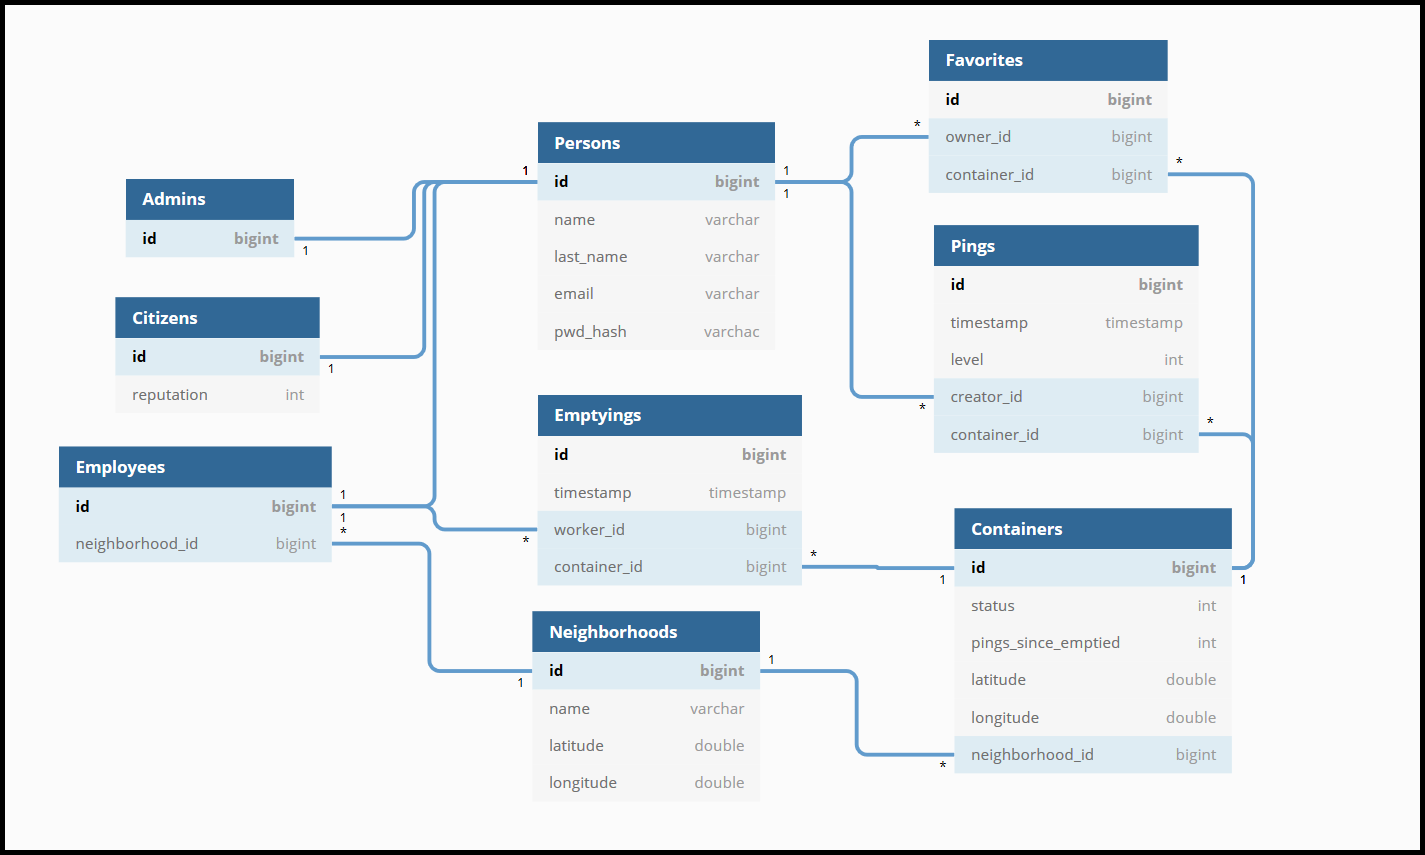
\includegraphics[scale=0.5]{figures/db_diagram.PNG}
					\centering
					\caption{Dijagram baze podataka}
					\label{fig:db-diag}
				\end{figure}
			
				\begin{figure}[H]
					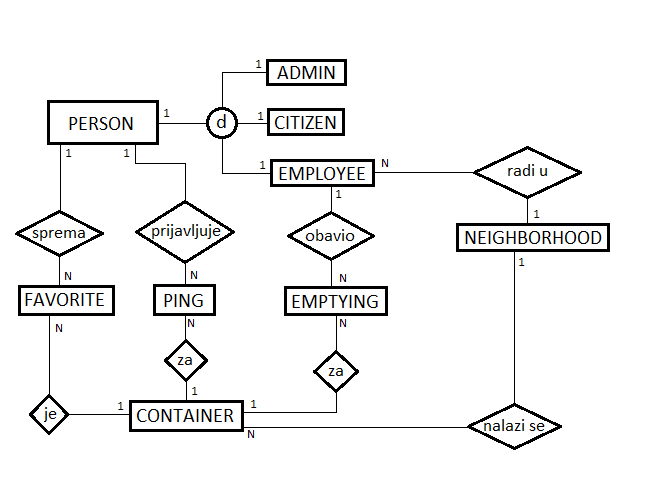
\includegraphics[scale=0.8]{figures/er_model.PNG}
					\centering
					\caption{Entitetsko-Relacijski model baze podataka}
					\label{fig:er-model}
				\end{figure}
			
			\eject
			
			
		\section{Dijagram razreda}
		
			Slika 4.5 prikazuje dijagram razreda koji predstavljaju model podataka - reprezentaciju stvarnog svijeta. On je vrlo sličan ER modelu i dijagramu baze podataka, ali ne i identičan: uspoređujući ih, vidljivo je kako se Java objekti i sve veze (One-to-one, One-to-many, Many-to-many) mapiraju u bazu podataka.
			
			Na slici 4.6. prikazan je dijagram razreda paketa \textit{dao}. DAO (\textit{Data Access Object}) je paket koji predstavlja sloj između logike aplikacije i baze podataka. Pomoću DAO objekata aplikacija dohvaća objekte iz baze podataka te ih uključuje u razne akcije, mijenja, stvara nove objekte vezane uz njih i sprema ih natrag u bazu. Sve metode u svim razredima ovog paketa su već implementirane u Spring-ovom sučelju JpaRepository, koje sva naša sučelja nasljeđuju.
			
			Slika 4.7 prikazuje dijagram razreda paketa \textit{controller}, koji su zaduženi za primanje HTTP zahtjeva na način da se svaka metoda u pojedinom \textit{controller} razredu mapira na određeni URL i određenu HTTP metodu (GET, POST, PUT...). Tako je primjerice metoda registerUser() u razredu PublicController pozvana isključivo ako korisnik pošalje POST zahtjev na URL "/register", a metoda testAuthorization() se koristi kako bi korisnik provjerio ispravnost autorizacijskih podataka slanjem GET zahtjeva na URL "/auth". 
			
			Konačno, svaki razred iz prethodnog paketa sadrži referencu na barem jedan razred iz paketa \textit{service} sa dijagrama na slici 4.8. Razredi ovog paketa su servisi koji obavljaju poslovnu logiku aplikacije, pružajući uslugu razredima iz paketa \textit{controller}, a koristeći razrede iz paketa \textit{dao}. Servisi često osim na repozitorije imaju i reference na druge razrede iz istog paketa.
			
			
			\begin{figure}[H]
				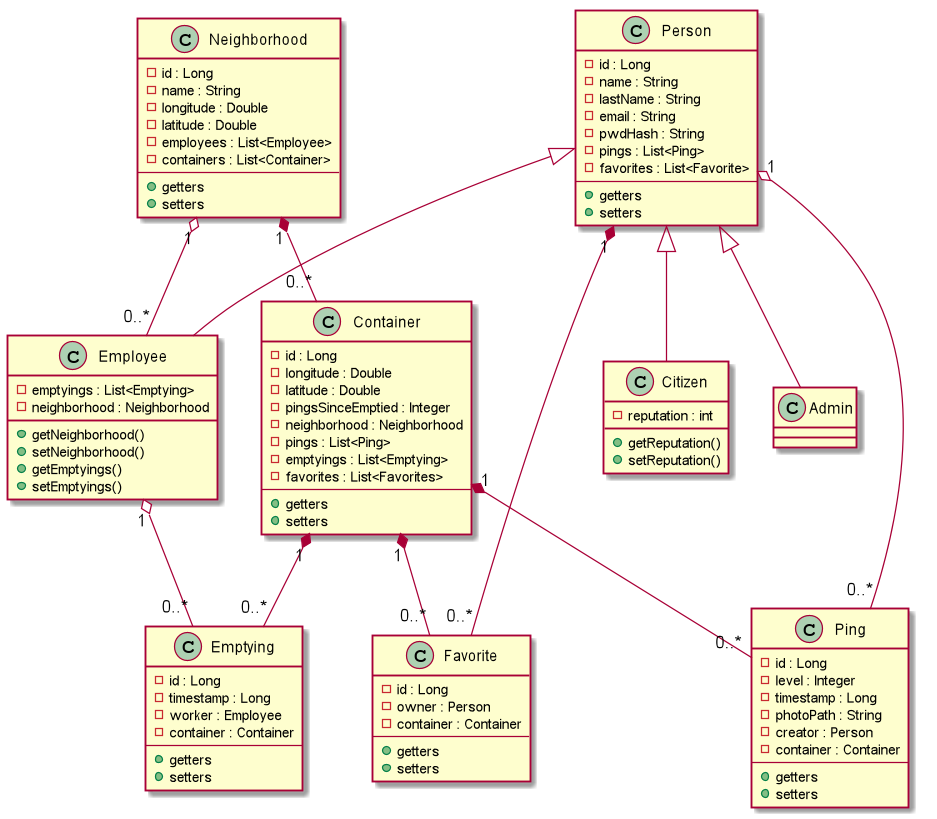
\includegraphics[scale=0.5]{figures/ModelClassDiagram.PNG}
				\centering
				\caption{Dijagram razreda koji predstavljaju model podataka}
				\label{fig:model-cd}
			\end{figure}
		
			\begin{figure}[H]
				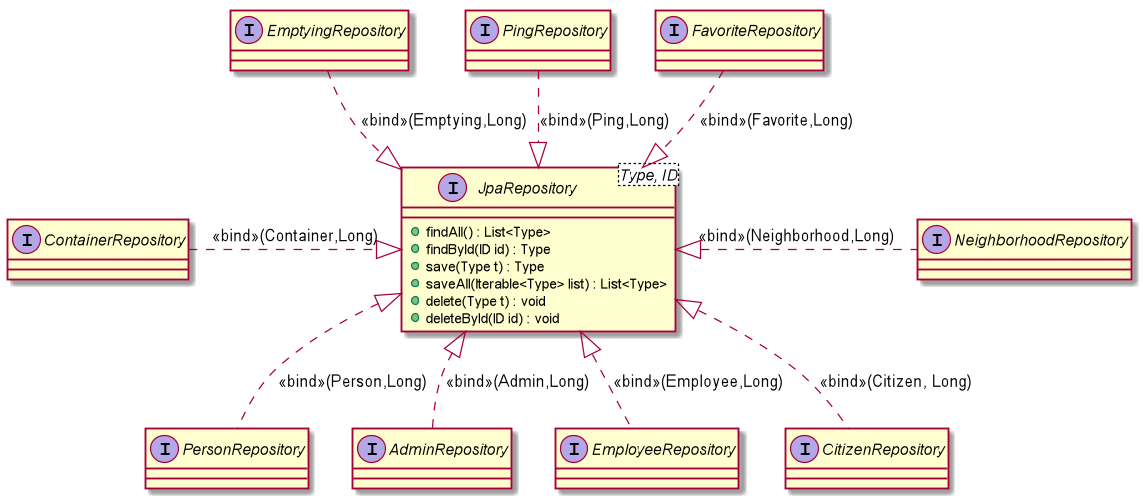
\includegraphics[scale=0.4]{figures/DAOClassDiagram.PNG}
				\centering
				\caption{Dijagram razreda paketa DAO}
				\label{fig:dao-cd}
			\end{figure}
		
			\begin{figure}[H]
				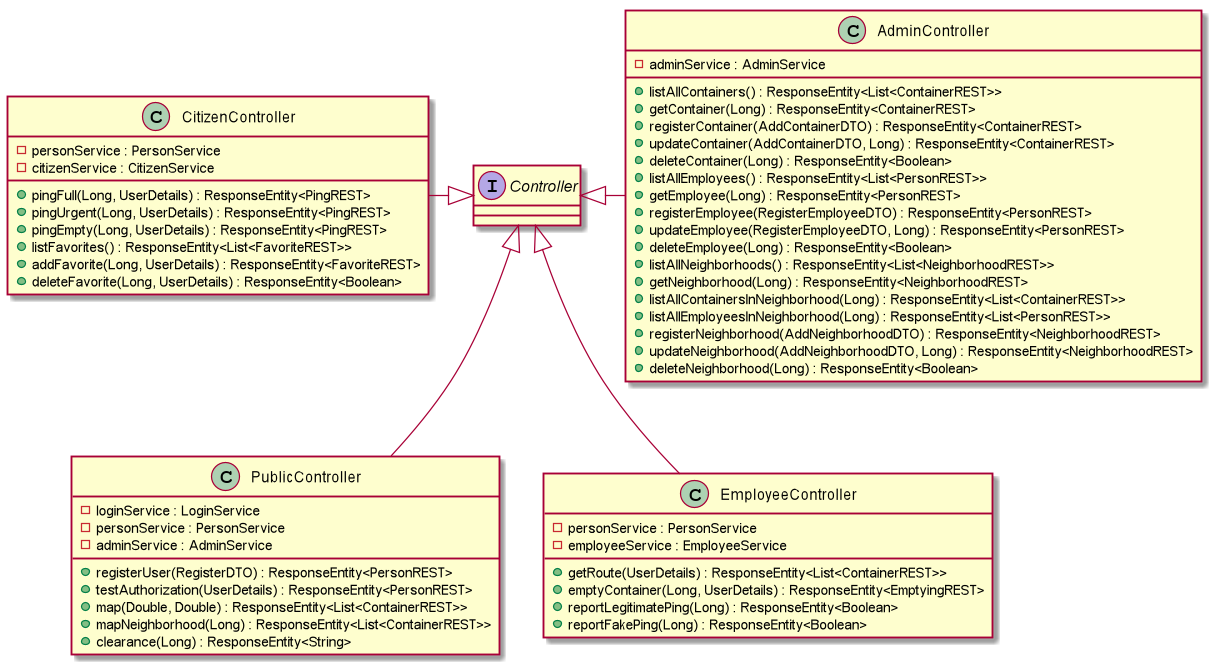
\includegraphics[scale=0.35]{figures/ControllerClassDiagram.PNG}
				\centering
				\caption{Dijagram razreda paketa controller}
				\label{fig:controller-cd}
			\end{figure}
		
			\begin{figure}[H]
				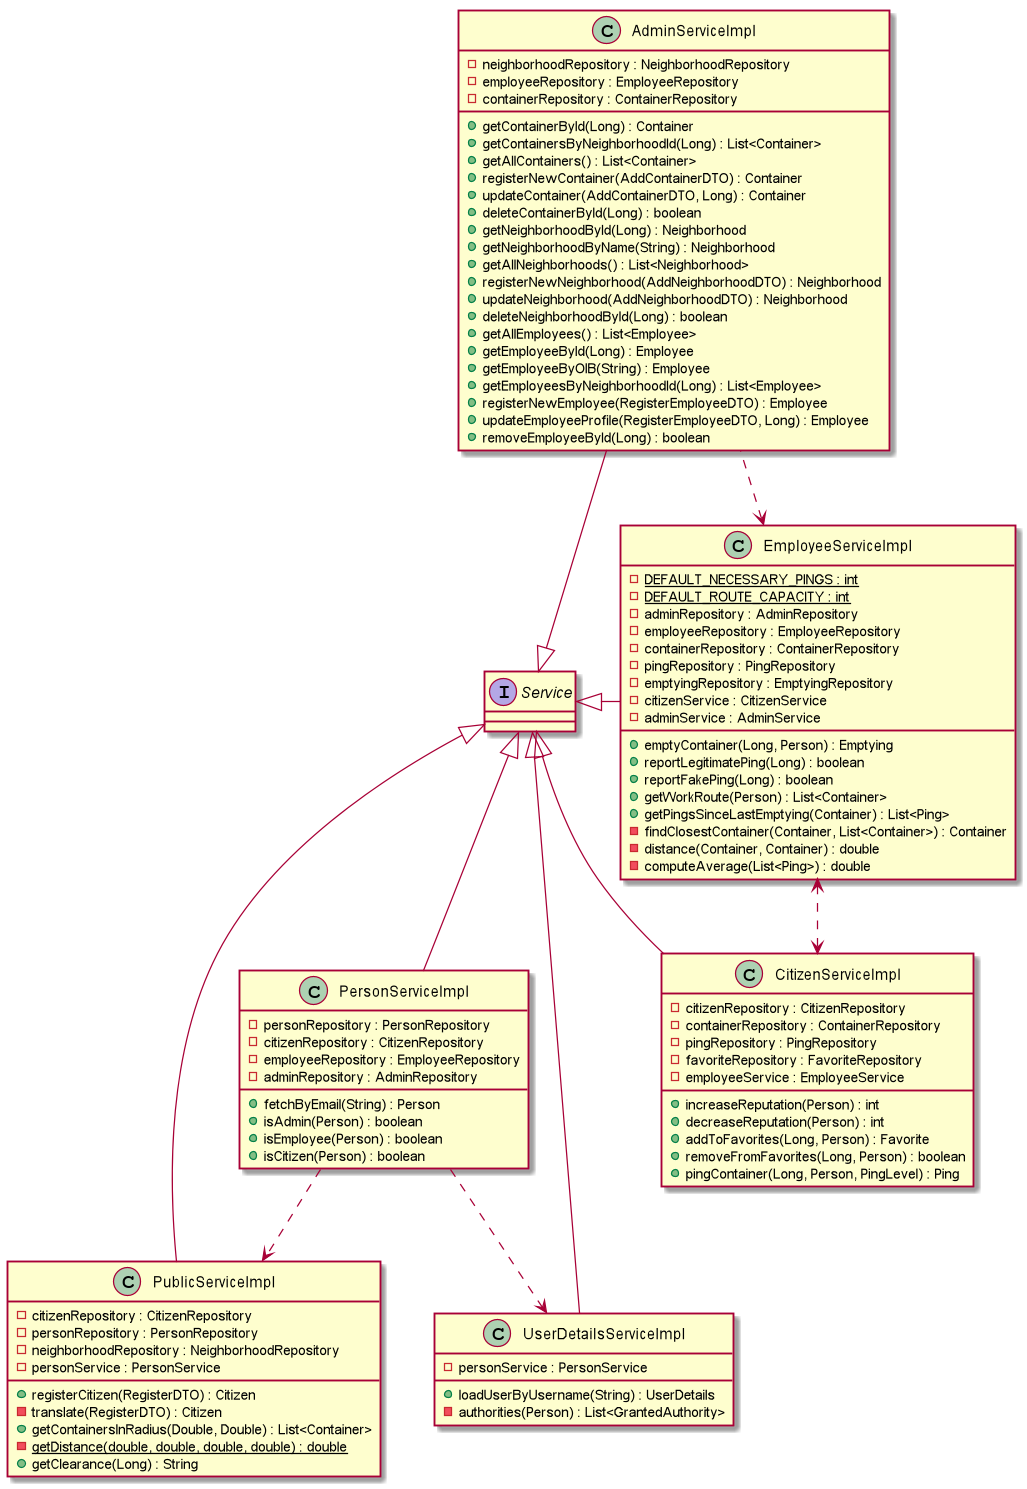
\includegraphics[scale=0.35]{figures/ServiceClassDiagram.PNG}
				\centering
				\caption{Dijagram razreda paketa service}
				\label{fig:service-cd}
			\end{figure}
			
			\eject
		
		\section{Dijagram stanja}
		
		Dijagram stanja prikazuje stanja objekta te prijelaze iz jednog stanja u drugo temeljene na dogadajima. Na slici 4.9 prikazan je dijagram stanja za registriranog
korisnika. Nakon prijave, građaninu se prikazuje početna stranica na kojoj može pregledati kartu i kontejnere. Za odabrani kontejner ima opciju prijavljivanja stanja kontejnera. Dodatno može priložiti i sliku prijavljenom stanju. Također, klikom na "Omiljeni kontejneri" prikaz naglašava prethodno označene najkorištenije kontejnere te tako olakšava prijavu stanja te iste može i obrisati ili dodati nove. Odabirom datuma i pripadnog željenog područja prikazuje se stanje karte za dotični datum na tom mjestu ukoliko traženi zapis postoji.
			
			\begin{figure}[H]
				\includegraphics[scale=0.4]{figures/Dijagram stanja - građanin.PNG}
				\centering
				\caption{Dijagram stanja}
				\label{fig:Dijagram stanja}
			\end{figure}
			
			\eject 
		
		\section{Dijagram aktivnosti}
			
			Dijagram aktivnosti primjenjuje se za opis modela toka upravljanja ili toka podataka. Ne upotrebljava se za modeliranje dogadajima poticanog ponasanja. U modeliranju toka upravljanja svaki novi korak poduzima se nakon zavrsenog prethodnog, a naglasak je na jednostavnosti. Na dijagramu aktivnosti 4.10 prikazan je proces prijave stanja kontejnera. Građanin se prijavi u sustav i odabere kontejner za kojeg želi prijaviti stanje. Zatim mu se prikazuje popis opcija za prijavu te on bira koje stanje želi prijaviti. Nakon što potvrdi odabir sustav mu vraća potvrdu o uspješnoj prijavi.
			
			\begin{figure}[H]
				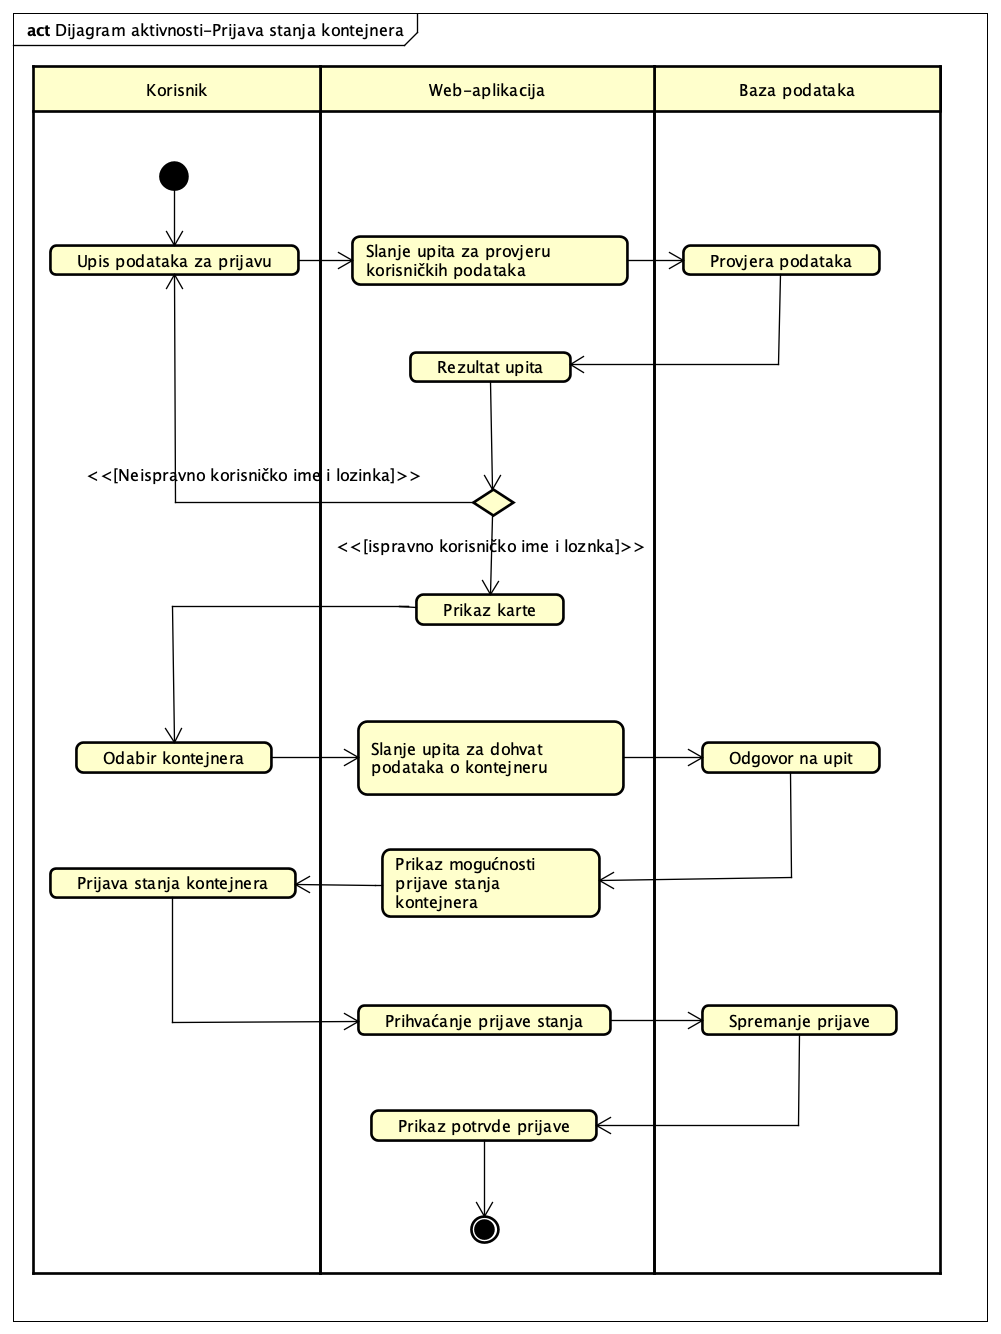
\includegraphics[scale=0.4]{figures/Dijagram aktivnosti-Prijava stanja kontejnera.PNG}
				\centering
				\caption{Dijagram stanja}
				\label{fig:Dijagram_aktivnosti}
			\end{figure} 
			
			
			\eject
		\section{Dijagram komponenti}
		
			Dijagram komponenti služi za prikaz komponenti koje tvore sustav, njihove organizacije i međuovisnosti. Na slici 4.11 prikazan je dijagram komponenti za programsku potporu koju smo razvili. Aplikacija je, najgrublje gledano, podijeljena na tri strogo odvojene cjeline: 
			\begin{packed_item}
				\item \textit{Frontend aplikacija} pokrenuta na jednom NGINX poslužitelju i na kojoj se nalaze statički resursi poput HTML stranica, JavaScript modula te CSS datoteka pomoću kojih su sve HTML stranice dizajnirane.
				\item \textit{Manje Smeće Više Sreće aplikacija} pokrenuta na Tomcat poslužitelju u kojoj se nalazi sama implementacija aplikacije podjeljena na razine \textit{Controller}, \textit{Service}, \textit{Repositories}, \textit{Model} i \textit{DTO}. Svaka od tih razina čini jedan neizostavni dio aplikacije.
				\item \textit{PostreSQL Baza Podataka} pokrenuta na zasebnom poslužitelju. U nju se spremaju svi podaci u obliku Java objekata pomoću JDBC/JPA specifikacije.
			\end{packed_item}
			
			Statičke HTML stranice određuju formu, a njihov izgled određen je CSS \textit{stylesheetovima} na istom poslužitelju. Za dinamičko dohvaćanje podataka s \textit{backenda} kao i njihov prikaz ugradnjom u HTML koriste se JavaScript moduli. U modulima obuhvaćenim grupom \textit{AJAX Requests} nalazi se po jedna metoda za svaku metodu u svim razredima \textit{Controller}, time omogućujući jednostavno spajanje na REST API i dohvat podataka u JSON formatu.
			
			\begin{figure}[H]
				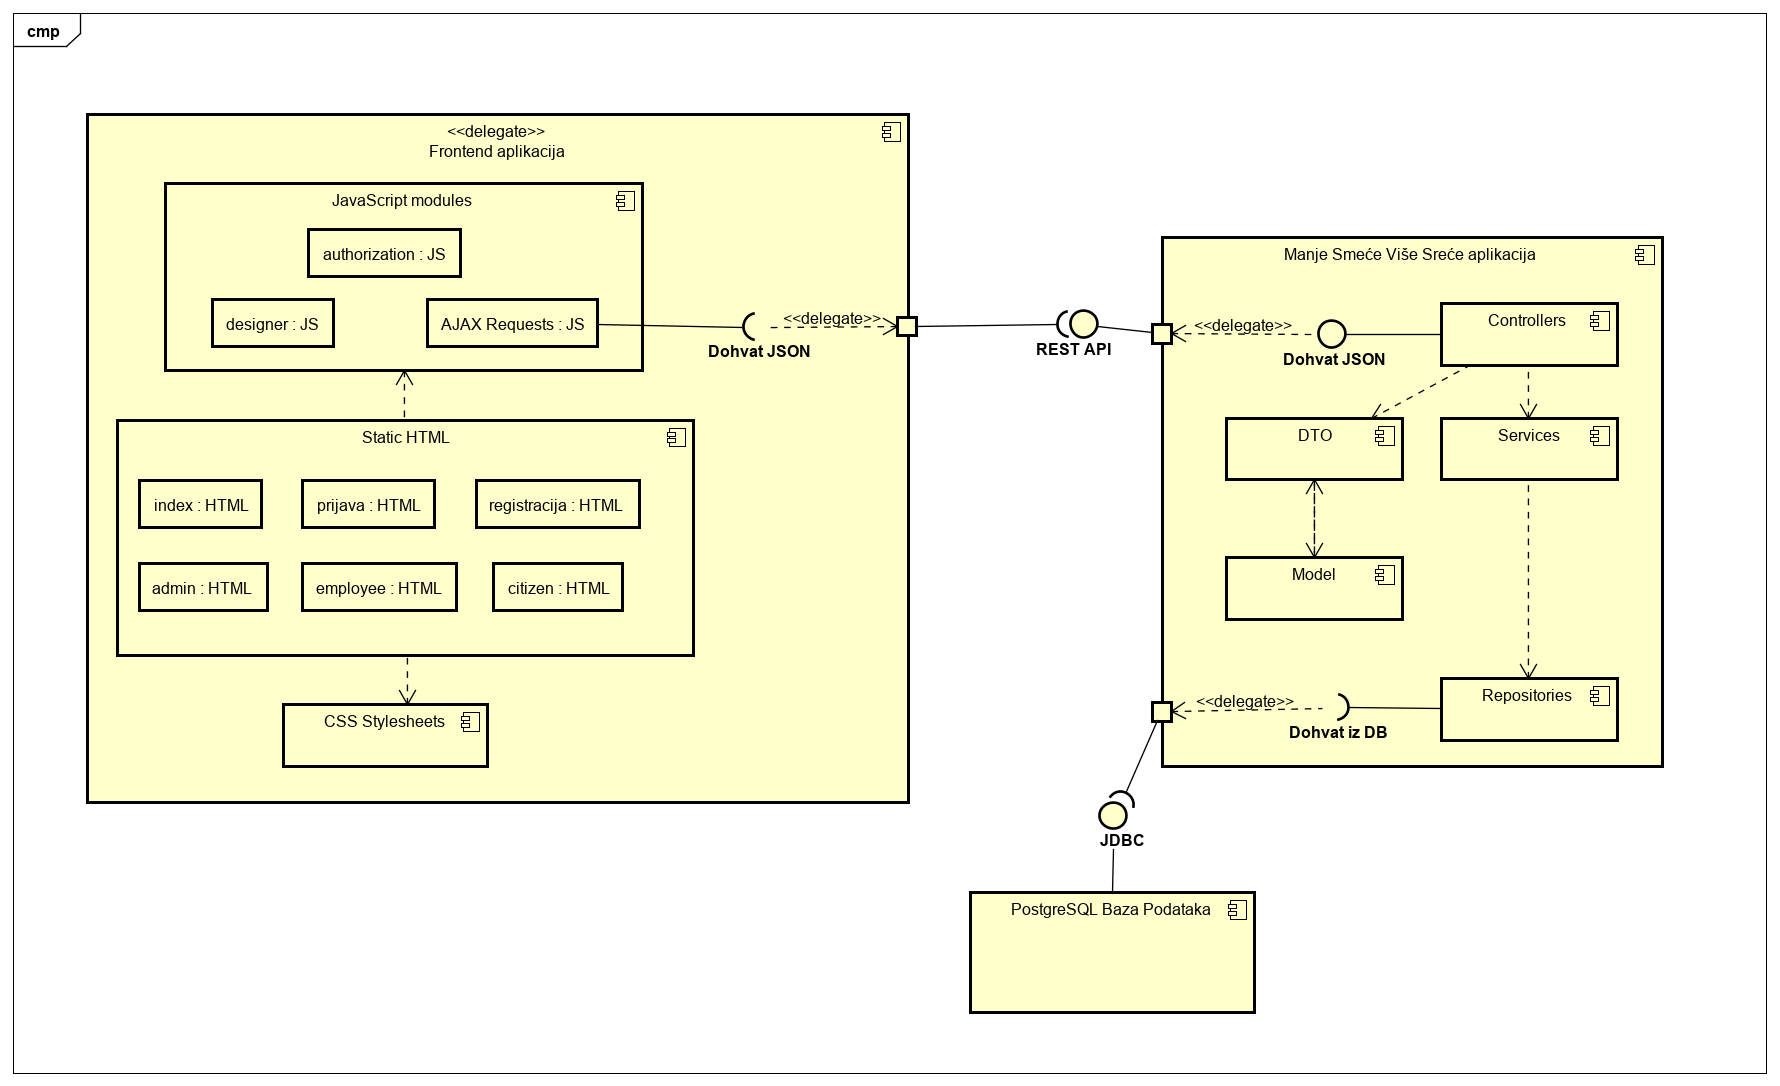
\includegraphics[scale=0.35]{figures/MSVSComponentDiagram.PNG}
				\centering
				\caption{Dijagram komponenti}
				\label{fig:komp-dijag}
			\end{figure} 
		